\documentclass[11pt,a4paper]{article}

\usepackage[margin=1in]{geometry}
\usepackage{titlesec}
\usepackage{enumitem}
\usepackage{hyperref}
\usepackage{parskip}
\usepackage{graphicx}
\usepackage{float}
\usepackage{xcolor}
\usepackage{booktabs}
\usepackage{ragged2e}

\hypersetup{
    colorlinks=true,
    linkcolor=blue,
    urlcolor=blue
}

\titleformat{\section}{\large\bfseries}{\thesection}{0.5em}{}
\titleformat{\subsection}{\normalsize\bfseries}{\thesubsection}{0.5em}{}

\title{\vspace{-1.5cm}\textbf{PKCERT AI \& Software Development Internship \\ Task 06: Exploratory Data Analysis with a Jupyter Notebook}}
\author{Abdullah Amir}
\date{AI and Software Development \\ 09 July 2026}

\begin{document}

\maketitle
\vspace{-1cm}

\tableofcontents
\vspace{0.5cm}

% ======================================================================
\section*{Overview}
\addcontentsline{toc}{section}{Overview}
This report is the written companion to my Task 06 Jupyter notebook,
\texttt{EDA\_Wine\_Quality.ipynb}. The task was to take a real dataset, explore
it properly, and write up what the data is actually telling us. The notebook
does the hands-on work with markdown notes at every step, and this report pulls
the story together with the same figures and the key takeaways.

I picked the \textbf{Red Wine Quality} dataset from the UCI Machine Learning
Repository. It is a nice fit for an EDA exercise: every column is numeric, it has
a clear target to explain, and it has just enough data-quality quirks to be
realistic without being a mess.

% ======================================================================
\section*{Part A: The Dataset}
\addcontentsline{toc}{section}{Part A: The Dataset}
\begin{itemize}[leftmargin=1.4em]
    \item \textbf{Source:} UCI Machine Learning Repository, originally from
    Cortez et al. (2009).
    \item \textbf{Purpose:} Each row is a Portuguese red \emph{vinho verde}
    wine. Eleven physicochemical lab measurements were recorded, and a panel of
    tasters scored each wine. The question is whether the chemistry can explain
    the score.
    \item \textbf{Records:} 1,599 wines to start with.
    \item \textbf{Features (11, all numeric):} fixed acidity, volatile acidity,
    citric acid, residual sugar, chlorides, free sulfur dioxide, total sulfur
    dioxide, density, pH, sulphates, and alcohol.
    \item \textbf{Target:} \texttt{quality}, an integer taster score that runs
    from 3 to 8 in this data.
\end{itemize}

% ======================================================================
\section*{Part B: Exploratory Data Analysis}
\addcontentsline{toc}{section}{Part B: Exploratory Data Analysis}

\subsection*{Structure and Summary}
The table is 1,599 rows by 12 columns, and every column comes in as a number, so
there is nothing to decode or convert. The summary statistics show the columns
live on very different scales: total sulfur dioxide runs into the hundreds while
density sits right around 1.0. The quality score averages about 5.6, so most
wines are middling rather than brilliant or awful.

\subsection*{Data Quality}
The dataset is unusually tidy on missing values: there are none at all. It does
have \textbf{240 fully duplicated rows} though. Those might be genuinely
different wines that recorded identical measurements, but to keep them from
getting double weight I dropped them, which leaves \textbf{1,359 unique rows}.
There were no other inconsistencies to fix: every measurement is positive and
sits in a physically sensible range, for example pH between roughly 2.7 and 4.0,
which is exactly where wine should be.

\subsection*{Visualizations}
The notebook produces six figures, each with a short interpretation. They are
reproduced here.

\subsubsection*{1. Distribution of the quality score}
\begin{figure}[H]
    \centering
    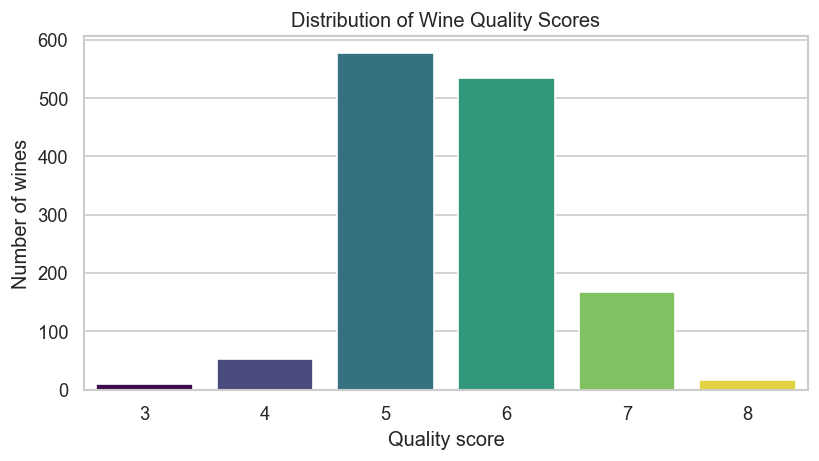
\includegraphics[width=0.68\textwidth]{figures/01_quality_distribution.png}
    \caption{How many wines sit at each quality score.}
\end{figure}
The scores pile up on 5 and 6, with very few wines at 3, 4, or 8. This imbalance
is worth remembering: there simply are not many examples of great or poor wines
to learn from.

\subsubsection*{2. Distribution of each chemical feature}
\begin{figure}[H]
    \centering
    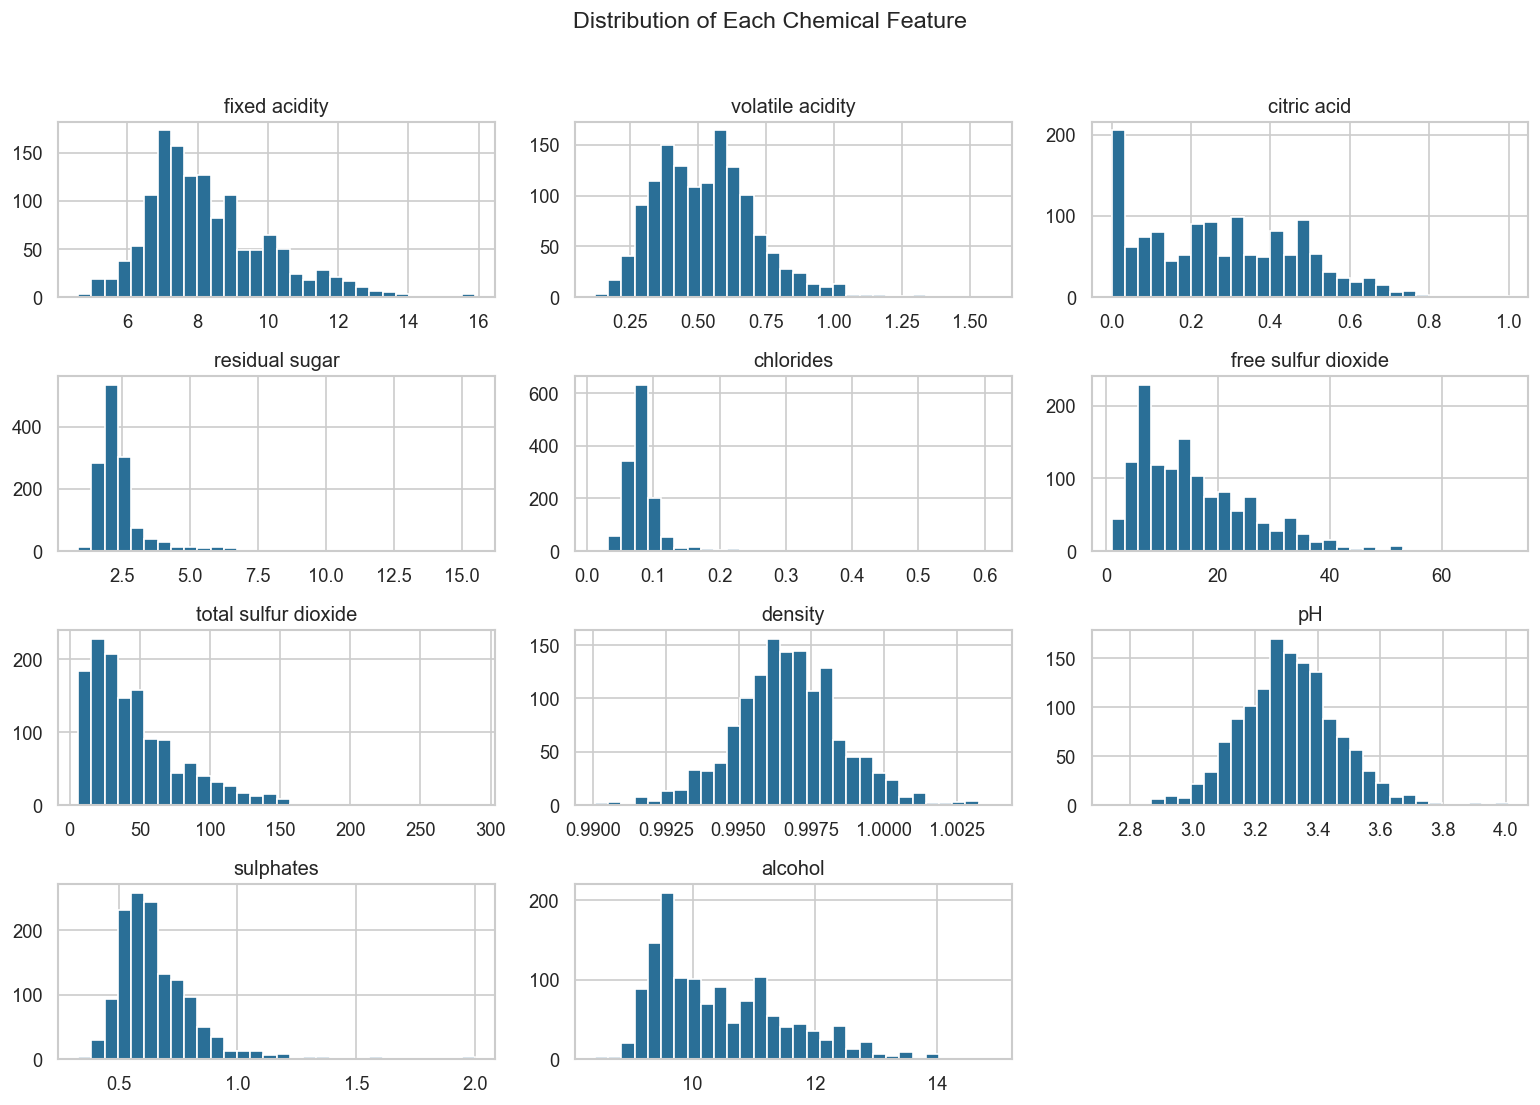
\includegraphics[width=0.92\textwidth]{figures/02_feature_histograms.png}
    \caption{Histograms of all eleven features.}
\end{figure}
Most features are right skewed with a long tail of high values. Residual sugar
and chlorides are the most extreme, with a few wines sitting far out to the
right. That skew is a hint that a handful of wines are chemically unusual and
that scaling would help before any modelling.

\subsubsection*{3. Correlation heatmap}
\begin{figure}[H]
    \centering
    
\includegraphics[width=0.82\textwidth]{figures/03_correlation_heatmap.png}
    \caption{Correlation between every pair of features.}
\end{figure}
This is the most useful single view. Reading the quality row, alcohol has the
strongest positive correlation (about +0.48) and volatile acidity the strongest
negative one (about -0.40). Among the features themselves, fixed acidity ties to
citric acid and density, and the two sulfur dioxide columns move together, all
of which is chemically sensible.

\subsubsection*{4. Alcohol by quality}
\begin{figure}[H]
    \centering
    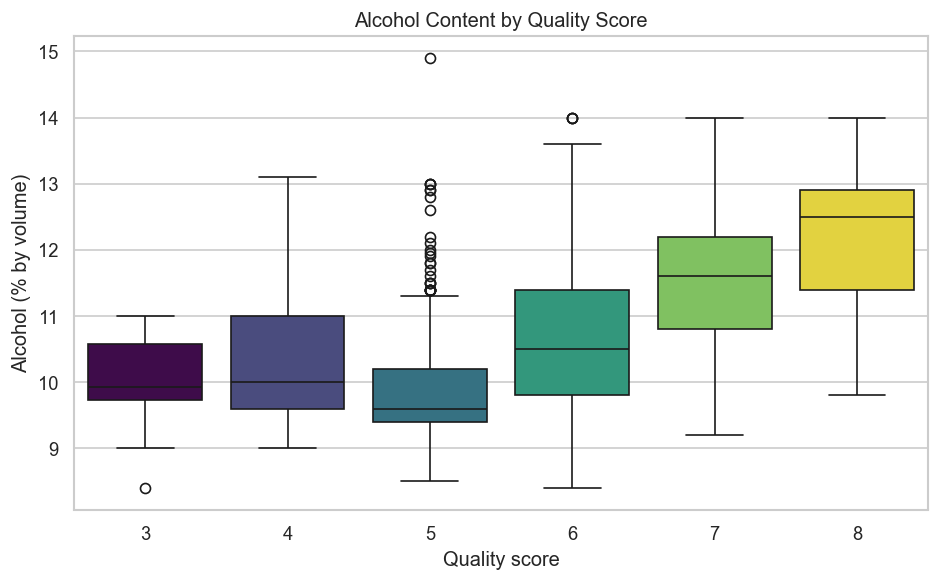
\includegraphics[width=0.72\textwidth]{figures/04_alcohol_by_quality.png}
    \caption{Alcohol content for each quality score.}
\end{figure}
This is the clearest relationship in the data. From score 5 upward, the median
alcohol content climbs at every step, so better rated wines tend to be more
alcoholic. It is the same signal the heatmap flagged, now easy to see.

\subsubsection*{5. Volatile acidity by quality}
\begin{figure}[H]
    \centering
    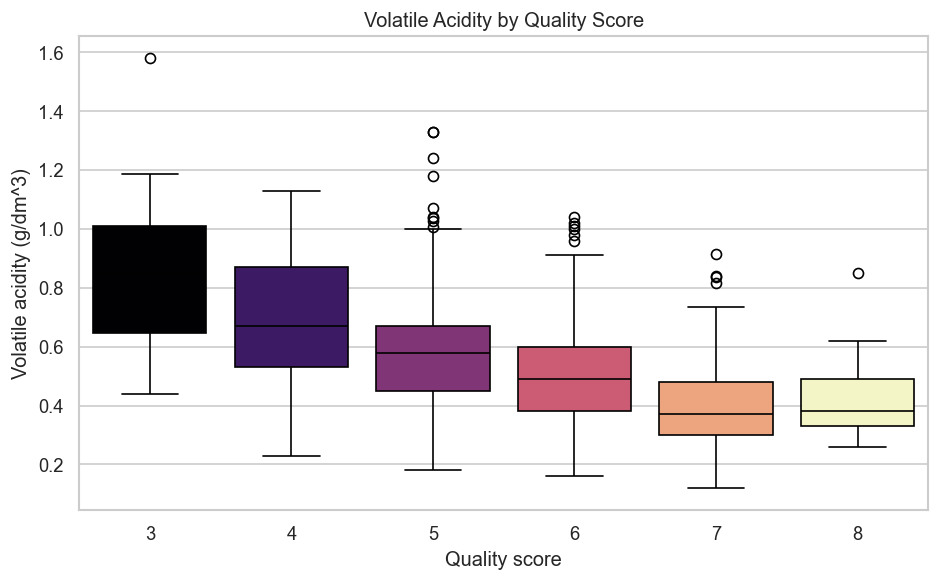
\includegraphics[width=0.72\textwidth]{figures/05_volatile_acidity_by_quality.png}
    \caption{Volatile acidity for each quality score.}
\end{figure}
This chart is the mirror image of the last one. Volatile acidity is what gives
wine a sharp vinegar note, and its median drops as quality rises. Tasters
clearly marked down the more acidic wines.

\subsubsection*{6. Correlation of each feature with quality}
\begin{figure}[H]
    \centering
    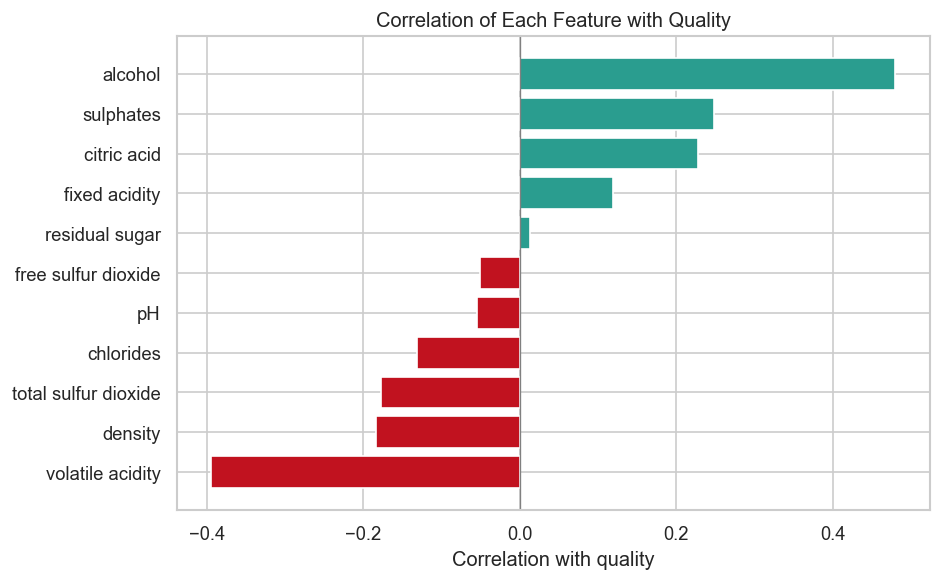
\includegraphics[width=0.72\textwidth]{figures/06_correlation_with_quality.png}
    \caption{Every feature's correlation with the quality score.}
\end{figure}
Lining the numbers up in one bar chart gives a tidy summary. Alcohol, sulphates,
and citric acid help a wine's score, while volatile acidity hurts it the most,
followed by total sulfur dioxide, density, and chlorides. Everything else sits
close to zero.

% ======================================================================
\section*{Part C: Findings and Insights}
\addcontentsline{toc}{section}{Part C: Findings and Insights}

\subsection*{Key Findings}
\begin{itemize}[leftmargin=1.4em]
    \item Quality rides on just a few features: alcohol (positive) and volatile
    acidity (negative) are by far the two biggest signals, with sulphates and
    citric acid adding a smaller positive push.
    \item Higher alcohol goes hand in hand with higher ratings.
    \item Sharp, acidic wines score badly.
    \item The target is imbalanced, with most wines rated 5 or 6.
\end{itemize}

\subsection*{What This Could Mean}
For a winemaker, the practical read is that aiming for a strong fermentation
(higher alcohol) while keeping volatile acidity low is the chemical combination
most tied to a better score. Sulphates, which work as a preservative, also line
up with slightly better ratings. From a research angle, no single feature
correlates above about 0.5 with quality, which says the rating is genuinely a
multi-factor thing. That points towards a model that combines features rather
than leaning on any one measurement.

\subsection*{Limitations and Next Steps}
The biggest limitation is the class imbalance: with so few wines at the extremes,
it is hard to say much about what makes a wine truly great or truly poor. The
target is also subjective, since quality is an average of human taste scores. And
because these are all red \emph{vinho verde} wines from one region, the findings
may not carry to other wines. A natural next step would be to fold in the white
wine dataset for a bigger and more balanced picture, group the scores into low,
medium, and high to ease the imbalance, and then train a classifier to see how
well the chemistry actually predicts quality on unseen wines.

% ======================================================================
\section*{Part D: Notebook Organization}
\addcontentsline{toc}{section}{Part D: Notebook Organization}
The notebook is laid out to follow this same structure. It opens with the
dataset description, moves through the exploratory analysis (structure, data
quality, then the visualizations with a note under each), and closes with the
written insights. Markdown headings separate every stage, the code cells are
commented, and each figure is explained right where it appears. All the charts
are saved into the \texttt{figures/} folder, which is how they made their way
into this report.

The full project, including the notebook, the dataset, the figures, and this
report, is on my GitHub repository for the internship:
\url{https://github.com/AbdullahAmir06/ai-internship-abdullahamir}.

% ======================================================================
\end{document}
